%%% For details on how to use this template see file "readMe"

\documentclass{def/tuberlin}
\usepackage{amsthm}
\usepackage{amsmath}
\usepackage{amssymb}
\usepackage{caption}
\usepackage{graphicx}
\usepackage{bbm}
\usepackage{placeins}

% Figures live in the talk's image folder one level up
\graphicspath{{../}{./}}


\theoremstyle{definition}
\newtheorem{definition}{Definition}[section]
\newtheorem{theorem}{Theorem}[section]
\newtheorem{example}{Example}[section]
\theoremstyle{remark}
\newtheorem*{remark}{Remark}

\author{Loay Hefni
	\and Jonas Persé 
	% \and (First name(s)) (Last name)
	% \and First name(s)) (Last name)
}
\usepackage{lipsum}

\title{Scoring Rules for Probabilistic Forecasting}
\subtitle{Summary of the Seminar-Talk } 

% choose *one* document type
% \documentType{Journal article}
%\documentType{Book chapter}
%\documentType{Conference paper}

% \documentType{Preprint}
%\documentType{Report}

% Optional for Reports: enter project/funding info -- in language of the title. Examples: "DFG-Abschlussbericht, Projekt: 462163815" or "Final report DFG project: [GEPRIS-Nr.]"
%\fundingAck{DFG-Abschlussbericht, Projekt: 123456789}


%\documentVersion{\submitted} %% any author-created version that has been submitted for publication and is still under review
% \documentVersion{\accepted} %% final author-created version as accepted for publication
%\documentVersion{\published} %% final publisher-created version as published

%\dateOfVersion{...} % to specify the date when this version was created/last edited

% \versionAvailableAtDOI{10.[xxx]} % specify the DOI where this open access version will be available 

%  use https://citation.doi.org/ to create a citation string
% \citationDetails{Doe, Jane; Doe, John (Year). Title of the publication: subtitle if applicable. Journal, Volume(Issue), PageStart--PageEnd. \url{https://doi.org/10.[xxx]}.}
% if applicable, remember to escape the ampersand character ("\&") in list of authors!


%\publisherStatement{Some publishers require a specific statement, if applicable include it here}
% for Preprints: can be used to include further infos on status, e.g. "submitted to $journal ($date)" or "under review, submitted to $journal (ISSN: xxx)

% to specify which user rights are granted for the open access version ("In Copyright" recommended for otherwise closed access works, see further info in "readMe" file)
% \termsOfUse{\InCopyright}
%\termsOfUse{\CCBYlic}
%\termsOfUse{\CCBYSAlic}
%\termsOfUse{\CCBYNDlic}
%\termsOfUse{\CCBYNClic}
%\termsOfUse{\CCBYNCSAlic}
%\termsOfUse{\CCBYNCNDlic}

\begin{document}    
\tuberlintitle

\tableofcontents

\newpage

\chapter{Introduction}
In our talk we looked at so-called Scoring Rules for Probabilistic Forecasting as a means of assigning a score to a prediction made by some sort of machine learning algorithm. These predictions are usually given in a probabilistic setting, i.e. not as deterministic values, but rather as a cumulative distribution function or as a density function. A Scoring Rule then assigns a numerical value to a prediction, based on the predicted density, distribution, etc. and the real value that is observed. In the talk, we discussed the different settings in which Scoring Rules can be defined and used. Starting the talk, we gave the intuition behind Scoring Rules before introducing the rigorous mathematical definition. Overall, the talk was close in structure to the paper \cite{Gneiting} by first introducing categorical scores, giving examples like the Brier Score, Logarithmic Score and Zero-One-Score. For the chapter on continuous scores the focus mainly lies on the Logarithmic Score and the Continuous Ranked Probability Score (CRPS), giving examples of when these might be useful. Further, we also discussed Kernel Scores as a way to quickly recover Scoring Rules via negative definite kernels and Scoring Rules for quantiles, in which case there no longer is some sort of predictive distribution function, but rather certain sections of the underlying distribution are predicted.

\newpage
\chapter{Scoring rules for continuous forecasts}
A predictive distribution in a continuous setting can be given in the form of a predictive density or a predictive cumulative distribution function (CDF), which gives a motivation to look at scoring rules for both ways of giving a forecast in this setting. This chapter is closely related to the corresponding chapter in \cite{Gneiting}, adding some examples to illustrate the practical use of certain scoring rules.
\section{Scoring rules for predictive densities}
Let $\mu$ be a $\sigma$-finite measure on some measurable space $(\Omega,\mathcal A)$. Let $\mathcal L_\alpha, \alpha>1$ be the set of probability measures $P$ on $(\Omega,\mathcal A)$, which are absolutely continuous with respect to $\mu$, such that the $\mu$-density $p$ of $P$ satisfies the following condition: \begin{align*}
    \lVert p\rVert_\alpha = \left(\int p(\omega)^\alpha \mu(d\omega)\right)^\frac{1}{\alpha}<\infty.
\end{align*}
\begin{remark}
    The $\mu$-density of a probability measure is not uniquely defined; however, \cite{Gneiting} references a way to uniquely determine a certain $p$ for some $P$ in $\mathcal{L}_\alpha$ when needed.
\end{remark}
Given this, scoring rules can be defined on the sets $\mathcal L_\alpha$ for certain values of $\alpha$.
\begin{definition}[quadratic score]
    The quadratic score is defined as \begin{align*}
        \text{QS}(p,\omega)=2p(\omega)-\lVert p\rVert_2^2,
    \end{align*}
    where $p$ is the given predictive density we want to score and $\omega$ is the real value that materialized. This scoring rule is strictly proper with respect to $\mathcal L_2$.
\end{definition}
\begin{definition}[logarithmic score]
    The logarithmic score is defined as \begin{align*}
        \text{LogS}(p,\omega)=\log p(\omega)
    \end{align*}
    and is strictly proper relative to the class $\mathcal L_1$, which is the class of measures dominated by $\mu$.
\end{definition}
A more general scoring rule, which is not restricted to a single value of $\alpha$, is given by the following definition 
\begin{definition}[pseudospherical score]
The pseudospherical score is given by \begin{align*}
    \text{PseudoS}(p,\omega)=\frac{p(\omega)^{\alpha-1}}{\lVert p\rVert_\alpha^{\alpha-1}}
\end{align*}
and is strictly proper relative to the class $\mathcal L_\alpha$.
\end{definition}
\subsection{Using the logarithmic score}
Because of its simplicity, the logarithmic score is widely used in various different settings. A particular and also possibly problematic use case of the logarithmic score was described in \cite{Candela} and \cite{Kohonen}. In this particular case, a variation of the logarithmic score was used in a so called PASCAL challenge to score predictions given by an algorithm in the form of a density function. In this challenge, the predictive density was used to estimate the relation between two variables. Utilizing the logarithmic score in this scenario, however, came with a problem. If it was reasonable to expect some point on the continuous space of possible outputs for the given input to have a point mass (a probability greater than $0$), one could pick a small interval around this value and set the density on this interval as shown in Fig. 2.1. Since the logarithmic score only depends on the value at the observed point $\omega$, hitting the interval with an almost arbitrarily high density would result in a very high score, even when averaging over multiple observations.
\begin{figure}[h]
    \centering
    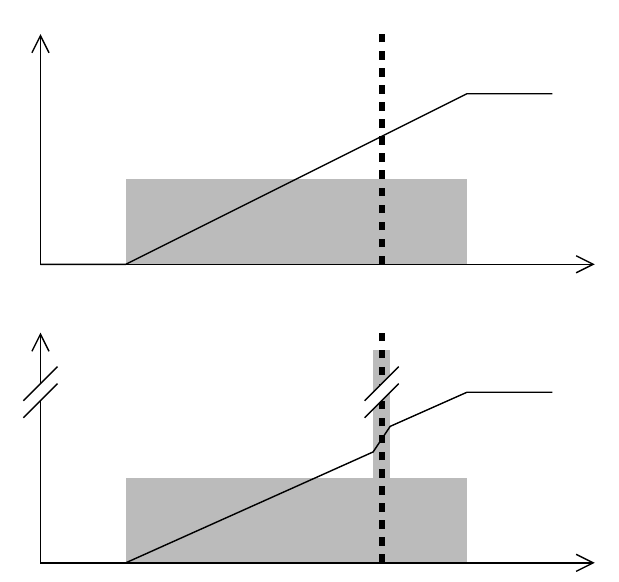
\includegraphics[width=0.5\textwidth]{images/Graphic Kohonen Suomela.png}
    \caption{Figure 8 of \cite{Kohonen} shows how small intervals can have very high densities without altering the corresponding CDF very much}
    \end{figure}
\section{Scoring rules for CDF}
As seen in the previous chapter, relying only on predictive densities can be a problem, as in the example of the PASCAL challenge. Problems like this could be prevented if CDFs were used instead of predictive densities. Besides that, using a CDF would also allow one to use discrete measures on sample sets to represent the predictive distribution more easily, as shown in Fig 2.2. Using the logarithmic score with the same representation would result in an "infinite penalty" if a value outside the sample materializes.
\begin{figure}[!h]
            \centering
            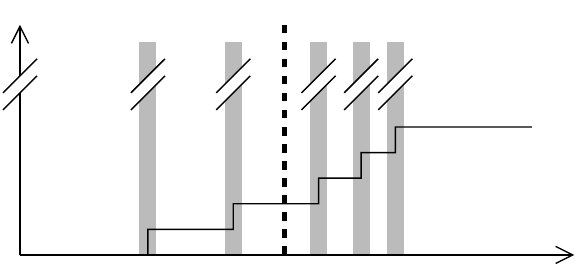
\includegraphics[width=0.5\linewidth]{images/Kohonen Suomela Fig.9.png}
            \caption{ Figure 9 of \cite{Kohonen} shows how a discrete distribution on samples can be used to approximate a CDF}
            \label{fig:placeholder1}
\end{figure}
\subsection{Continuous Ranked Probability Score (CRPS)}
\begin{definition}[CRPS]
    Let $\mathcal P$ be the set of Borel probability measures (measures defined on the Borel $\sigma$-algebra) on $\mathbb R$. Then we define the Continuous Ranked Probability Score as \begin{align*}
        \text{CRPS}(F,x)=-\int_{-\infty}^\infty (F(y)-\mathbbm 1_{\{y\geq x\}})^2 dy
    \end{align*}
\end{definition}
Fig. 2.3 shows that the CRPS can be interpreted as a way of measuring the area between the predictive CDF and the point measure at the materialized value.
\begin{remark}
The CRPS is proper with respect to $\mathcal P$ and strictly proper with respect to the class $\mathcal P_1$ of Borel probability measures with finite first moments.
\end{remark}
\begin{remark}
    The divergence function connected to the CRPS is defined by \begin{align*}
        d(F,G)=\int_{-\infty}^\infty (F(y)-G(y))^2dy
    \end{align*}
\end{remark}
Another useful characteristic of the CRPS is the consideration of "distance" in the sense that, if an algorithm predicts a point measure in some point, the CRPS would give a higher score to measures in points closer to the materialized value than ones farther away, which can also be seen in Fig. 2.3. to some extent.\begin{figure}[h]
    \centering
    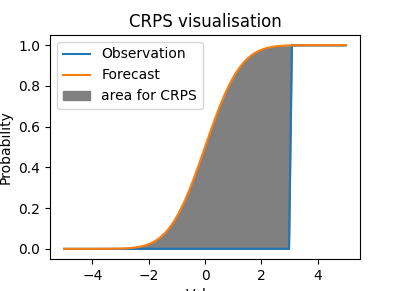
\includegraphics[width=0.5\linewidth]{images/Figure_3.png}
    \caption{Visualization of the area used in the CRPS if the forecaster gives the CDF of a normal distribution with mean at $0$ and the materialized value is $3$}
    \label{fig:placeholder2}
\end{figure}
\begin{remark}
    The CRPS can also be defined as \begin{align*}
        CRPS(F,x)=\frac 12 E_F[\lvert X-X'\rvert]-E_F[\lvert X-x\rvert]
    \end{align*}
    where $X,X'$ are independent copies of a random variable with distribution $F$
\end{remark}
\subsection{Considering other scores}
After focusing strongly on the CRPS, it remains to be said that the CRPS has the downside that the integral needed to compute the score is not always easy to calculate. Therefore, as stated in \cite{Gneiting}, one might have to resort to numerical methods to compute it. Other scores that can be considered instead of the CRPS are the so-called energy score, which is a generalization of the CRPS to $\mathbb R^n$, or scores based only on the first and second moments of distributions.
%\chapter{Preliminaries}
%\section{Mathematical Background}
\chapter{Kernel scores}
In this chapter we look at the question of how scoring functions can be easily defined using so-called kernels, and we look at some examples of using those kernels to recover some of the scores we already know.
\begin{definition}[negative definite kernel]
Let $\Omega$ be a nonempty set and let $g$ be a real valued function on $\Omega\times\Omega$. If $g$ is symmetric, i.e., $g(x,y)=g(y,x)$ and \begin{align*}
    \sum_{i=1}^n\sum_{j=1}^n \alpha_i\alpha_j g(x_i,x_j)\leq 0
\end{align*}
    for all positive integers $n$, all $\alpha_1,\dots,\alpha_n\in\mathbb R$ that sum up to $0$ and all $x_1,\dots,x_n\in\Omega$, then $g$ is called a negative definite kernel.
\end{definition}
Having defined what a kernel is, we now get the following theorem connecting negative definite kernels and scoring rules:
\begin{theorem}
Let $\Omega$ be a Hausdorff space and let $g\colon\Omega\times\Omega\to\mathbb R$ be a non-negative and continuous negative definite kernel. If now $P$ is a Borel probability measure on $\Omega$ and $X,X'$ are independent with distribution $P$, the expression \begin{align*}
    S(P,x)=\frac 12 E_P[g(X,X')]- E_P[g(X,x)]
\end{align*}
is a proper scoring rule with respect to the class of Borel probability measures on $\Omega$.
\end{theorem}
The proof of the Theorem is outlined in \cite{Gneiting}.
\begin{example}
    Take $g(x,x')=\lvert x-x'\rvert$ as a negative definite kernel. Using the theorem, we get the alternative definition of the CRPS.
\end{example}
\begin{example}
    Let $\Omega =\{0,1\}$ and let $g(0,0)=g(1,1)=0, g(1,0)=g(0,1)=1$. If we again use the theorem we get the Brier score as the resulting scoring function.
\end{example}
\section{Further results}
It is also possible to consider complex valued kernels defined in a similar manner. By doing so, it is possible to define a generalized version of the theorem from before. By doing this and choosing a fitting complex kernel, we can get \begin{align*}
    -\int_{\mathbb R^m}\lvert \phi_P(y)-e^{i\langle x,y\rangle}\rvert^2\mu(dy).
\end{align*}
Under certain conditions on $\mu$ this scoring rule is strictly proper relative to the class of Borel probability measures on $\mathbb R^m$.
\chapter{Scoring rules for quantiles}
In the previous chapters, we looked at scoring rules for a given density or cumulative distribution function. In some cases, however, it might not be useful to look at a whole distribution and it might be enough to know where certain sections of the distribution lie. This motivates the following definition: 
\begin{definition}[quantiles]
For use in this chapter, we consider quantiles $r_1,\dots,r_k$ at the levels $\alpha_1,\dots,\alpha_k\in (0,1)$ to be values such that \begin{align*}
    P(x\leq r_k)=\alpha_k
\end{align*}
\end{definition}
\begin{remark}
    Since the values described as in the definition are, in general, not unique, we assume that our underlying Borel probability measure $P$, besides other assumptions, has a strictly increasing distribution function.
\end{remark}
With this definition, we look at scoring functions of the form $S(r_1,\dots,r_k,x)$, where $r_1,\dots,r_k$ are the predicted quantiles and $x$ is the materialized value. We then call a scoring rule proper if \begin{align*}
    S(q_1,\dots,q_k,P)\geq S(r_1,\dots,r_k,P)
\end{align*}
for all real numbers $r_1,\dots,r_k$, if $q_1,\dots,q_k$ are the real quantiles of $P$.
\begin{theorem}[Thm 6 in \cite{Gneiting}]
    Let $s$ be a nondecreasing function and $h$ be arbitrary, then \begin{align*}
        S(r;x)=\alpha s(r)+(s(x)-s(r))\mathbbm 1_{\{x\leq r\}}+h(x)
    \end{align*} 
    is proper for predicting a single quantile at level $\alpha\in(0,1)$.
\end{theorem}
\begin{proof}
    Assume $r<q$, then \begin{align*}
        S(q;P)-S(r;P)&=\int \alpha s(q)+(s(x)-s(q))\mathbbm 1_{\{x\leq q\}}+h(x)-(\alpha s(r)+(s(x)-s(r))\mathbbm 1_{\{x\leq r\}}+h(x))\,dP(x)\\
        &=\int\alpha s(q)-\alpha s(r)+(s(x)-s(q))\mathbbm 1_{\{x\leq q\}}-(s(x)-s(r))\mathbbm 1_{\{x\leq r\}}\, dP(x).
    \end{align*}
    Dividing the integral into parts over the sets $(-\infty,r],(r,q),[q,\infty)$ gives that the above expression is equal to \begin{align*}
        \int_{(r,q)}s(x)\, dP(x)+s(r)P(r)-\alpha s(r)&\geq\int_{(r,q)}s(r)\, dP(x)+s(r)P(r)-\alpha s(r)\\
        &=s(r)\bigl(P(q)-P(r)\bigr)+s(r)P(r)-\alpha s(r)\\
        &=s(r)P(q)-\alpha s(r)\\
        &=0,
    \end{align*}
    where the inequality holds because $s$ is nondecreasing, so $s(x)\geq s(r)$ for all $x\in(r,q)$, and the last equality holds because $P(q)=\alpha$ by the definition of the quantile $q$. Hence $S(q;P)\geq S(r;P)$.
    For $r>q$ the argument is analogous, concluding the proof.
\end{proof}
\section{Use cases of quantiles} 
In financial mathematics, it might be reasonable trying to find the highest possible loss on an investment excluding the lowest 1\% of outcomes as unreasonable. This concept is connected to the so called Value at Risk which by different sources is considered to be the 1\% quantile of density on possible financial loss or the expected loss on an investment excluding the lowest 1\% of possible losses. The latter definition is visualized in Figure 4.1 \begin{figure}
    \centering
    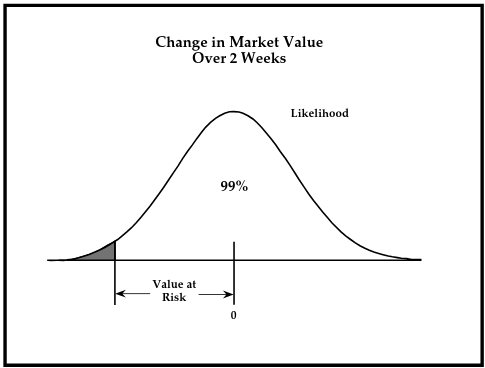
\includegraphics[width=0.5\linewidth]{images/VaR.png}
    \caption{Figure one of \cite{VaR} of the Value at Risk defined as some kind of expected value}
    \label{fig:placeholder3}
\end{figure}
\chapter{Further application of scoring rules}
In this chapter, we will briefly discuss the intention behind using scoring rules to compare forecasting models to each other. Consider $X=(X_1,\dots,X_n)$ to be the values supposed to be forecast by some forecasting model. The goal is to use scoring rules as a way of comparing different forecasting models, as stated in the beginning. Until now, we considered forecasts to be fully specified. We now change this assumption and consider the forecasting rules we are looking at to be specified up to a parameter $\theta$. Consider $H_k, k\in\{1,\dots,n\}$ to be one of $n$ forecasting models. Using the logarithmic score on the so called integrated likelihood we get: \begin{align*}
    S_{k,B}=\sum_{t=1}^n \log P(X_t\mid X^{t-1},H_k).
\end{align*}
Since we are now looking at likelihood, the probability a value receives from the model $H_k$ depends on the values $X^{t-1}$ that the model previously had to predict (we assume the values $X_1,\dots,X_n$ are in a particular order for this to work). From this point on, one could invent further scoring rules and ways to compare models, which we skipped in the presentation because it would require too much time.
\nocite{Unger}
\bibliographystyle{plain}
\bibliography{../References/refs}
\end{document}